\documentclass{interim}
\usepackage{graphicx}

% alternative font if you prefer
%\usepackage{times}

% for alternative page numbering use the following package
% and see documentation for commands
\usepackage{fancyheadings}

% make links clickable
\usepackage[hidelinks]{hyperref}

% get degree symbols
\usepackage{gensymb}

% superscript for dates
\newcommand{\ts}{\textsuperscript}

% allow custom labels for lists
\usepackage{enumitem}

% enable styled captions
\usepackage[format=plain,
labelfont={bf},
textfont=it,tableposition=above]{caption}


% other potentially useful packages
%\uspackage{amssymb,amsmath}
\usepackage{url}
\usepackage{fancyvrb}
\usepackage[final]{pdfpages}

\begin{document}

%%%%%%%%%%%%%%%%%%%%%%%%%%%%%%%%%%%%%%%%%%%%%%%%%%%%%%%%%%%%%%%%%%%
\title{Title of project placed here}
\author{Lewis Trundle}
\date{15th December 2023}
\maketitle
%%%%%%%%%%%%%%%%%%%%%%%%%%%%%%%%%%%%%%%%%%%%%%%%%%%%%%%%%%%%%%%%%%%

%%%%%%%%%%%%%%%%%%%%%%%%%%%%%%%%%%%%%%%%%%%%%%%%%%%%%%%%%%%%%%%%%%%
\tableofcontents
\newpage
%%%%%%%%%%%%%%%%%%%%%%%%%%%%%%%%%%%%%%%%%%%%%%%%%%%%%%%%%%%%%%%%%%%

%%%%%%%%%%%%%%%%%%%%%%%%%%%%%%%%%%%%%%%%%%%%%%%%%%%%%%%%%%%%%%%%%%%
\section{Introduction}\label{intro}
\subsection{Motivation}
Each year, road-traffic accidents account for 1.35 million deaths worldwide, with cyclists comprising 41,000 of these fatalities \cite{world2018global}. The economic burden associated with road accidents in the EU alone is estimated to amount to 236 billion euros annually \cite{costoftransport}. Despite the EU achieving an average annual reduction of 3\% in motor vehicle related fatalities, between 2010 and 2018, the fatality rate for cyclists remained the same across that same period \cite{adminaite2020safe} - emphasising the lack of attention towards cyclists regarding road safety.

One of the leading causes of fatalities among cyclists are collisions with a motorised vehicle \cite{BIL20101632}, with 78\% of cyclists fatalities in the EU due to bicycle-to-vehicle collisions \cite{adminaite2015making}. Although a collision with another vehicle may occur from any angle, those where the offending vehicle crashes from behind the cyclist causes the largest proportion of fatalities of all crash directions \cite{BIL20101632}. Despite a large body of research investigating how cyclist safety can be improved using safety systems implemented within other road vehicles \cite{scholliers2014potential, SILLA2017134, cieslik2019improving, 7929602, 10.1145/3434770.3459732} relatively few studies have explored how cyclist safety can be improved from the perspective of the cyclist \cite{10.1145/3490099.3511127, STROHAEKER2022151}. 

Cycling is often considered to be a task which requires a large amount of cognitive effort. Studies investigating the cognitive demand of cycling has shown that novice cyclists often struggle to accomplish cognitive tasks which are necessary for traffic safety \cite{https://doi.org/10.1002/acp.2350050205}. To aid cyclists, safety technology such as rear-view bike radars \cite{garminradar}, help reduce cognitive load, by delivering warning message both visually and audibly on approaching vehicles from behind. An obvious benefit of auditory messages is that they do not consume the visual sensory channel of the cyclist. However, auditory messages have been shown to be difficult to understand in noisy environments \cite{noisyenv} and in situations such as when the cyclist is listening to music, something which many admit to doing \cite{DEWAARD2011626}.

A possible alternative message modality is vibro-tactile, something which has typically only been used in cycling for navigational purposes \cite{10.1145/2371574.2371631, 10.1145/1613858.1613911}. Regarding where to encode vibro-tactile stimulation, there are many options. Many previous works have used belts \cite{10.1145/1613858.1613911, 10.1145/1463160.1463179, tsukada2004activebelt, 10.1145/2449396.2449450, 10.1145/1060581.1060585}, vests \cite{729547, 998954, van2000tactile}, and even the hands [cite all] as mediums for vibrational stimuli. Bicycles themselves have also been used \cite{10.1145/2371574.2371631, 10.1145/3290605.3300850}, with products such as attachable handlebar grips which can provide vibro-tactile feedback \cite{smartgrips}. However, a relatively unexplored area is the potential of the helmet. Few studies have explored how helmets can be used for interaction while cycling \cite{10.1145/2559206.2574803, 10.1145/1240866.1241027}, and fewer have investigated how they can be used to deliver vibro-tactile cues [cite all].

\subsection{Problem Statement and Aim}
Following our motivation, we formulate the specific problem which we aim to solve. That is, we aim to develop a device which can improve cycling safety - helping to lower the number of cyclist fatalities. More specifically, we aim to develop a hazard notification system for cyclists, able to effectively communicate to the cyclist when a vehicle from behind is approaching. 

The system is restricted to the context of notifying of vehicles behind the user, as from our motivation, this is deemed to be a possibly dangerous situation, with relatively little existing work to aid cyclists in this context. By focusing our system to work in this specific context, we aim to make the most impact in terms of improving cyclist safety.

Regarding developing this system, we first aim to investigate what is the best metric (or metrics) to convey to a cyclist, to appropriately inform them of approaching vehicles. We hypothesise that this would simply be \textit{distance}. However, categories of such a metric can be arbitrary - what specific distance does the term \textit{far} or \textit{near} mean to a cyclist? We hope to distinguish such meanings in this project.

Secondly, we aim to explore how this information can be encoded using vibro-tactile feedback. This modality is chosen due to its potential to provide feedback with minimal distraction. Therefore, our chosen coding method should be able to accurately represent the appropriate metric, with minimal diversion of the cyclists' attention. Furthermore, we explore how this system can be incorporated into a helmet - our chosen medium due to the relatively unexplored potential of bicycle helmets for interaction. We seek to answer which are the best places on the helmet to place vibro-tactile motors, and what parameters of the vibrations are most suitable for our system.

Finally, we aim to evaluate the system in a real-world user study, to learn cyclists' thoughts regarding its usefulness for cycling in real-life. By testing the system in realistic conditions, we hope to discover if it achieves its purpose of improving cycling safety.


%%%%%%%%%%%%%%%%%%%%%%%%%%%%%%%%%%%%%%%%%%%%%%%%%%%%%%%%%%%%%%%%%%%
\section{Background Survey}
There is little literature on hazard notification systems for cyclists, and of the existing corpus, few relate to the problem of cars encroaching from behind (the context in which this project is based). To address this issue, we first survey existing literature related to cycling safety, before examining literature regarding \textit{in-vehicle} hazard notification systems for cyclists. We then combine this with insights gathered from the use of different feedback modalities in cycling, as well as how vibro-tactile stimuli can be used to encode information, to form an overall view of how we can develop our proposed system.

\subsection{Hazard Notification for Cyclist Safety}
The idea of a hazard notification system was first explored in 1992 by Horowitz and Dingus \cite{doi:10.1177/154193129203601320}. They proposed various design approaches, such as adjusting the warning intensity based off the detected collision time, and employing different signal modalities to convey various warning severities - concepts which have been often used in later research. However, it was not until 1996 where one of the earliest hazard detection systems emerged \cite{566402}. While not explicitly labelled as a hazard detection system, this project combined radar and vision technologies to create a system which could detect and classify road vehicles ahead of the car, then appropriately change lanes to avoid collision. This idea of detecting vehicles in-front was continued in subsequent research by Huang et al. who developed a warning system which could detect lane boundaries and successfully detect a vehicle in-front with 97\% accuracy \cite{1307429}. Despite previous concerns about the effectiveness of imperfect in-vehicle collision avoidance warning systems, Ben-Yaacov \cite{doi:10.1518/0018720024497925} and Maltz and Shinar \cite{doi:10.1518/hfes.46.2.357.37348} demonstrated through a prolonged study that even these imperfect systems could significantly aid drivers, as after a relatively short use of the system, participants were able to maintain longer and safer headways for at least six months.

These early in-vehicle warning systems are all examples of Intelligent Transport Systems (ITSs) - a series of information and communications technologies which aim to improve the safety of transportation \cite{its}. Despite research into various types of ITSs, relatively few technologies study how the safety of vulnerable road users (VRUs), such as cyclists, can be improved \cite{Scholliers2017}. Silla et al. performed a quantitative safety impact assessment of five different types of ITSs, to evaluate which has the greatest potential to improve cyclist safety \cite{SILLA2017134}. They found that by 2030, the Pedestrian and Cyclist Detection System + Emergency Braking (an in-vehicle system which uses detection sensors to detect pedestrians/cyclists in front of a forward moving vehicle to warn and automatically brake) would have the greatest effect. The PROSPECT project \cite{cieslik2019improving}, funded by the European Commission, further improves the effectiveness of detection systems. Not only is it able to detect VRUs, but it can also detect their intentions - allowing the vehicle to take pre-emptive measures (such as changing speed or course) to avoid a collision. Expected to be completed by 2025, this project is estimated to reduce the number of seriously injured people in the EU by anywhere up to 2,500 people by 2030.

Another promising ITS mentioned by Silla et al. \cite{SILLA2017134} is Bicycle to Vehicle communication (B2V) systems. Jenkins et al. created a system which could bring cyclists onto the US Connected Vehicles Program \cite{usdot} - an initiative designed to bring vehicles onto a Vehicle-to-Everything (V2X) network\footnote{The \textit{'Everything'} part of V2X refers to any entity which has an impact or can be impacted by a vehicle. Typically, this is a combination of Vehicle-to-Vehicle (V2V) and Vehicle-to-Infrastructure (V2I) networks. In this specific case, Jenkins et al. aims to also include a Vehicle-to-Cyclist (V2C) network.}. This was done by outfitting cyclists with a low-cost DSRC-WAVE\footnote{Dedicated Short-Range Communications for Wireless Access in Vehicular Environments (DSRC-WAVE) is currently one of the only ways to provide V2X networks, with high reliability and low latency.} solution which allowed them to receive basic safety messages. From this, they created a multimodal hazard notification system which would deliver these safety messages using audio and haptic cues. By varying signal parameters, they were able to create a unique vocabulary of cues which cyclists could learn. This was delivered via a standard smartphone speaker and Boreal Bikes’ smrtGRiPs \cite{smartgrips}. Although the paper does not describe exactly how these cues were coded, it does describe the five hazard categories used to decide which action to recommend to the cyclist - ranging from cautionary messages to suggesting immediate action.

Lujic et al. combines the idea of cyclist detection systems and connected networks, to create InTraSafEd5G \cite{10.1145/3434770.3459732}, a system which can predict when pedestrians and cyclists will enter a vehicles' blind spot at intersections. By installing nodes across various traffic lights around Vienna, the authors create an Edge network which is able to detect critical situations and deliver early warning messages to drivers in real-time using 5G. These warnings are delivered both visually and audibly to a driver’s mobile phone. This work highlights the potential of combining various types of ITSs to create a system which enhances cyclist safety. However, the described system only provides a single type of notification to the driver, only alerting them of whether a potential collision is possible. An improved system may deliver different types of notifications which is able to effectively communicate more information about the potential collision.

Despite the potential for improving cyclist safety using ITSs, pre-existing attitudes and perceptions affect the acceptance of such systems. Angelis et al. investigated how attitudes towards cyclists effect how likely a driver is to use an in-vehicle cyclist detection system \cite{de2017negative}. They found that drivers who already express a negative representation of cyclists are more unlikely to accept a new technology than those who do not. This is further explored by Berge et al. who studied acceptance from the perspective of the cyclist, exploring their beliefs and attitudes towards being equipped with human-machine interfaces (HMIs) for communication with smart-traffic \cite{berge2022cyclists}. Through analysis of questionnaire responses and interviews, the authors identified that cyclists were worried about using HMIs as the responsibility of safety would be imposed on themselves, regardless of whether a situation warrants they take immediate action. 


\subsection{Feedback Modalities in Cycling}
Wolfe et al. investigated the different types of distractions which cyclists commonly face, finding that auditory distractions were most common, followed shortly by visual ones \cite{wolfe2016distracted}. Despite relatively little research into \textit{‘distracted biking’} \cite{mwakalonge2014distracted} it is generally believed that cyclists’ use of mobile phones is at the root of the cause. Angelis et al. studied the relationship between smartphone usage while cycling and frequency of crashes, finding that the usage of a smartphone led to an increased crash risk \cite{doi:10.1080/19439962.2019.1591559}. With over half a surveyed population admitting to using their mobile device on every trip \cite{GOLDENBELD20121} and 17\% of the population admitting to using one during every ride \cite{goldenbeld2010use}, there have been calls to put legislation in place to prevent the use of smartphones while cycling \cite{banphoneuse}. However, notably, Angelis et al.'s study found that the link between smartphone usage and increased crash risk was not true for their female subsample, and only applied to their male subset. Although they recommend investigating this further, this finding is also backed by other studies exploring differences in cycling behaviours based on factors such as gender \cite{BEHNOOD201735}. Furthermore, the authors admit to limitations in their study, such as the unreliability of participants remembering crashes. While some studies have investigated ways to improve smartphone interaction while cycling to reduce distraction \cite{10.1145/3544548.3580971, 10.1145/3152832.3152871} other approaches have investigated alternative interaction modalities, which don’t make use of the visual sensory channel.

The concept of utilising different sensory channels to convey information is an idea studied by Wickens \cite{wickens1984processing} and Wickens and Liu \cite{doi:10.1177/001872088803000505}, who explored ‘Multiple Resource Theory’ - a model of human information processing which predicts that attention is a limited cognitive resource that can be allocated across different tasks and modalities. The model implies that multiple sensory channels can be used simultaneously (within the cognitive load of the individual), without any individual one degrading the processing performance of the human operator. Seeking to take advantage of this concept, Wickens suggests that tasks can be configured to utilise multiple sensory channels - exploiting the information-processing capabilities of the human operator.

In the context of cycling, multiple works would explore the potential of utilising such a model, by developing tactile displays to aid navigation. One of the earliest instances of this was by Pielot et al. who developed Tacticycle - a bicycle with a minimal set of navigational cues encoded into the handlebars, to guide tourists to points of interests \cite{10.1145/2371574.2371631}. Direction was encoded via the relative intensity across both handlebars. For example, a 45\degree{} angle to the right was indicated by 25\% intensity vibration in the left handlebar and a 75\% intensity vibration in the right. This coding method proved effective, as participants in a study were able to understand the tactile cues and none of them reported losing orientation. However, the authors acknowledge that their testing environment was geographically constraint, and that it was likely participants could find the correct way to their destination as long as they travelled roughly in the right direction. Steltenpohl and Bouwer created Vibrobelt - a vibro-tactile belt also developed to aid navigation while cycling \cite{10.1145/2449396.2449450}. By analysing the visual focus and spatial knowledge acquisition of participants, the authors found that the use of Vibrobelt increased participants ability to recall images from the route, but were generally slower at navigating and recalling the route - showing a lesser contextual understanding. Peeters et al. investigated response times of vibro-tactile cues during various levels of physical cycling exercise \cite{peeters2019vibrotactile}. By attaching vibro-tactile motors to participants' spine and thighs, they showed that vibro-tactile signals were perceivable in both a stationary position, and during diverse levels of physical effort. Furthermore, they showed that cyclists' reaction time to stimuli shortened as they were cycling with greater effort. However, the study does not investigate the tactile perception of other body parts while cycling, such as the head.

Strohaeker et al. investigated the effect of unimodal warnings on cyclists to prevent collisions, specifically comparing acoustic and vibro-tactile warnings \cite{STROHAEKER2022151}. The results found that warnings, especially acoustic, were effective at shortening response times to potential collisions. Though, vibro-tactile warnings could also be effective for a system which does not require urgent reactions from the cyclist. This study however, did not consider how multimodal warnings could be used. The effects of unimodal and multimodal cues would be investigated by Matviienko et al. who compared the effectiveness of delivering navigational instructions to child cyclists using visual, auditory, and vibro-tactile feedback \cite{10.1145/3290605.3300850, 10.1145/3229434.3229479}. 
Visual cues were delivered using a flashing light on the left and right side of a bicycle helmet, using two different colour of light to indicate the distance until the next turn. Auditory cues were delivered using a speaker built into the helmet, and vibro-tactile cues were delivered using the bicycles' handlebars - similar to Tacticycle \cite{10.1145/2371574.2371631}. Results from their study showed that unimodal cues were easier to recognise, so were best to indicate directions, but multimodal cues were best used to communicate when immediate action is required as it demonstrated shorter reaction times and better understandability. However, due to the sample size and age of the participants, the authors acknowledge that these findings may not be generalisable to the public. This finding is backed by Sawitzky et al. who compared different awareness message modalities for cyclists to avoid dooring\footnote{Dooring is a type of collision where a parked vehicle door suddenly opens onto the path of an incoming cyclist. It has received much attention of the past decade, with anti-dooring laws \cite{roadsafetyrules, highwaycode, illinoiscode} and studies investigating anti-dooring techniques \cite{large2018validating}.} \cite{10.1145/3490099.3511127, mti6010003}. The authors compared the effectiveness of using combinations of visual messages, auditory icons, and voice messages for delivering warning notifications. The results showed that participants generally preferred the multimodal combination of visual messages and auditory icons. The study does not provide any evidence for how tactile feedback could be used, but does suggest it be studied for future work.

Despite the potential of using different communication modalities while cycling, there are drawbacks to each. Waard et al. investigated the effect that listening to music had on a cyclist \cite{DEWAARD2011626}. They found that cyclists' auditory perception deteriorated when doing so, with 68\% of participants missing auditory cues. Notably, no negative effects were recorded when participants only used one earbud.
A possible way these effects could be reduced is by using bone conducting headphones\footnote{These differ from regular headphones in that instead of projecting air pressure waves directly into a wearers' ear, they instead use the cheekbones to transfer auditory signals directly to the cochlea \cite{littler1952hearing}.} \cite{wolfe2016distracted}. However May and Walker \cite{may2017effects} studied the use of bone conduction headphones, and found that when distractor sounds were played through them, a wearers' ability to localise critical environment sounds worsened.

Erdei et al, reported that the perception of vibro-tactile signals during cycling worsen in environments where the surface causes haptic interference \cite{erdei2020comparing, doi:10.1080/15389588.2021.1985113}. However, they also believed this could be overcame by adjusting how the vibro-tactile stimuli was delivered to the cyclist. Tacticyle \cite{10.1145/2371574.2371631} delivered vibrations through the handlebars as they believed, \textit{“these are the only parts of the bicycle that the rider constantly touches during the ride”}. This statement would be proven correct by Hochleitner et al. who studied how cyclists give input to a system whilst staying on the move - finding that cyclists like to keep their hands on the handlebars as much as possible \cite{10.1145/3152832.3152871}. Furthermore, Porcheron et al. further studied cyclists use of technology while cycling and through findings of an ethnographic study, they introduced the concept that the handlebars are a ‘zonal space’ \cite{10.1145/3544548.3580971}. This alluded to the possibility of increasing a potential stimuli vocabulary, by encoding information across various zones of the handlebars. Companies have even capitalised on the capabilities of the handlebars for vibro-tactile feedback, with products such as smrtGRiPs \cite{smartgrips} which can be attached to the handlebars of any bicycle.


\subsection{Encoding Information using Vibro-tactile Stimuli}
\subsubsection{Coding Direction}
Much early work utilising vibro-tactile stimuli would explore how tactile displays could be incorporated alongside visual displays, to extend a computer systems’ functionality. Pentland, investigated how tactile displays could be used in wearable computing - suggesting they could be used as directional displays to aid navigation \cite{629923}. Pentland would shortly realise this idea of a wearable navigational display less than a year later in 1998, where they developed an adjustable vest which provides directional navigational instructions via vibrations \cite{729547}. These directions were conveyed by vibrating a grid of motors - which were sewn into the back of the vest - in a specific pattern. For example, to indicate a right turn, the motors were activated sequentially, from left to right. Research into the design of such a haptic vest would continue over the years, including a study, investigating its efficiency in conveying directional instructions across different gravity conditions \cite{998954}. Although the study found that the perceived intensity of vibrotactile signals did not change across the varying conditions, it did comment on the effect that cognitive load has on a persons ability to interpret tactile signals - suggesting the need for further psychophysical experiments investigating haptic perception.

This method of communicating direction makes use of a vibro-tactile illusion known as ‘sensory saltation' - a phenomenon where successive pulses delivered to equidistant regions of a body part simulates the feeling of movement across the body part \cite{geldard1975sensory}. Authors author et al. and author et al., studied different types of sensory illusions, dividing haptic illusions into two types: sensory saltation, and funneling, where the tactor signal is perceived in the middle of two simultaneously activated tactors \cite{5710913, s150407913}. How spatial characteristics of vibro-tactile motors effect the perception of such illusions is investigated by Roger W., who proves that illusions such as sensory saltation are just as effective as veridical sensations at conveying directional information \cite{cholewiak2000generation}.

Much later research would continue investigating how vibro-tactile displays could be effectively used to provide navigational aids. Van Erp would introduce a new direction coding scheme where the on-body location of a localised vibration would indicate the direction of travel \cite{van2000tactile}. Using a haptic vest similar to \cite{729547}, they would instead attach motors in a 360\degree{} horizontal plane around the wearers body, allowing directions in a 360\degree{} circumference to be conveyed. The benefit of only requiring a linear array of motors would lead to these systems being implemented on smaller wearables, typically a belt \cite{10.1145/1463160.1463179, tsukada2004activebelt, 10.1145/2449396.2449450}. Van Erp would also later investigate the spatial resolution of such a system, suggesting users could effectively navigate using a spatial resolution of only 45\degree{} (1 motor in each cardinal and oblique direction) \cite{10.1145/1060581.1060585}. Quantitively proven to reduce cognitive load on the user \cite{VANERP2004247}. This method of communicating direction would become the norm for tactile navigational displays.

\subsubsection{Coding Distance}\label{sec:coding-distance}
Although a simple navigational system may only convey direction to a user, a more effective one would also typically convey an idea of distance \cite{burntt2002empirical}. Parameters to encode information is studied by van Erp, who explores spatial and temporal effects of vibro-tactile stimuli \cite{guidelines}. The paper serves as a set guidelines for implementing a vibro-tactile system and suggests that a vibro-tactile display affords four parameters which can be adjusted: the location, timing, frequency, and amplitude of a vibration. How parameters such as these can be used is described by Brewster and Brown \cite{10.5555/976310.976313}, who introduce \textit{Tactons} - structured, abstract messages, whose meaning is encoded using the parameters of cutaneous perception\footnote{Cutaneous perception refers to receptors under the surface of the skin. The cutaneous senses are multimodal and includes sensations of temperature, pressure, and vibration.}. The authors expand on the parameters suggested by van Erp, explicitly describing how temporal characteristics of a vibration, such as rhythm and duration can be used.

Previous studies have investigated how these parameters can be used to create coding schemes for distance. van Erp et al. investigated the effectiveness of different distance coding schemes to aid navigation for pedestrian participants \cite{10.1145/1060581.1060585}. Two main categories of distance coding schemes were used; the first was a monotonic relation between distance and rhythm - as the distance got smaller, the rhythm got faster. The second category was a three-phase model, which varied the delay duration between vibration pulses, depending on which phase of the navigation task the participant was in. Navigational directions were encoded by the location of the vibro-tactile motors on a belt which participants wore. Notably, there was no difference found in participant performance when comparing those with access to distance information, to those without - concluding that this may be due to the confounding of the distance information with the temporal resolution of the direction information. Straub et al. conducted a similar experiment, also using a vibro-tactile belt to perform navigational tasks with pedestrians \cite{5326374}. Three experiments were preformed to explore how the encoding of distance using the parameters of rhythm, intensity, and frequency, affected the walking speed of participants. Similarly to van Erp et al. \cite{10.1145/1060581.1060585}, no notable differences to walking speed were found. However, this is likely attributable to the confounding of parameters, as both rhythm and intensity are simultaneously varied in the experimental coding schemes.

The inconclusive findings from van Erp et al. \cite{10.1145/1060581.1060585} and Straub et al. \cite{5326374} identified a need to further explore how distance can be coded using temporal aspects of vibro-tactile stimulation, something which the skin is very sensitive to \cite{doi:10.1068/p5014}. McDaniel et al. utilised tactile rhythms to create a coding scheme to convey intimate, personal, interpersonal, and social distances to the blind \cite{10.1145/1520340.1520718}. The duration of a pulse was kept to a constant 50ms, but as the distance increased, the delay between pulses increased, similar to van Erp et al.'s monotonic scheme \cite{10.1145/1060581.1060585}. However, this experiment proved effective, and showed that given a small training period, users were able to effectively identify different tactile rhythms and associate them with their respective distances. Pielot et al. further studied distance encodings by developing a tactile display which presents the position and distance of other team members in a fast-paced 3D multiplayer game \cite{10.1145/1753326.1753581}. They compared rhythm-based, duration-based, and intensity-based schemes. Participants found their rhythm-based scheme the easiest to judge distance. Furthermore, they proved it was possible to accurately use vibro-tactile signals to convey distance in an environment with high cognitive demand. Asif et al. \cite{10.1145/1868914.1868923} further studied these parameters, but instead explored how they could be combined to compare three rhythm-based schemes: rhythm only, rhythm and intensity, and rhythm and duration\footnote{The rhythm only scheme decreased the number of pulses as the distance decreased, but the overall rhythm duration was kept constant, meaning the pulse duration also increased. The rhythm and intensity scheme was similar to the rhythm only scheme, but it additionally decreased the intensity and distance decreased. The rhythm and duration scheme also decreased the number of pulses as the distance decreased, but the pulse duration was kept constant, meaning the overall rhythm duration decreased.}. These schemes were used in-vehicle, to indicate different categories of distance until an approaching turn. The results found that the combination of rhythm and duration was the easiest for participants to learn and led to the smallest amount of navigational mistakes.


\subsection{Interacting using Helmets while Cycling}
[[Spatial Discrimination of Vibrotactile Stimuli Around the Head]] - info to do with vibro around head. Useful when talking about location coding schemes
\cite{10.1145/2559206.2574803, 10.1145/1240866.1241027}
[[https://oaktrust.library.tamu.edu/handle/1969.1/151968]]
[[http://personales.upv.es/thinkmind/dl/conferences/vehicular/vehicular_2020/vehicular_2020_2_20_38002.pdf]]
[[https://link.springer.com/chapter/10.1007/978-3-642-39802-5_3]]


%%%%%%%%%%%%%%%%%%%%%%%%%%%%%%%%%%%%%%%%%%%%%%%%%%%%%%%%%%%%%%%%%%%
\section{Proposed Approach}

state how you propose to solve the software development problem. Show that your proposed approach is feasible, but identify any risks.

\subsection{TactiHelm System Design}
\subsubsection{Helmet Design}\label{sec:helmet-design}
The current TactiHelm helmet builds off previous work from Vo et al. \cite{10.1145/3411763.3451580}. The inside lining of the helmet is equipped with 10mm diameter, three volt ERM coin cell tactile actuators (tactors), placed along the midline of the helmet. The exact number and spacing of these actuators is not yet defined; however, is explored more in our lab-based study discussed in Section \ref{sec:lab-study}. These actuators are driven by PWM signals from 0 to 3V generated by an Arduino Uno micro-controller \cite{arduinouno}. PWM can represent the use of an analogue signal \cite{kart2001pulse}, allowing us to more precisely vary the range of discrete values used to control the intensity of the tactile actuators. The Arduino Uno has six PWM pins, thus if we wish to vary the intensity of the actuators, we are limited to just six of them. The circuit is also equipped with an HC-06 Bluetooth module, to allow for remote control over the actuators. This Bluetooth module communicates using Bluetooth Classic \cite{hc06}. A diagram of the full circuit can be seen in Figure 1.

\begin{figure}[!ht]
    \centering
    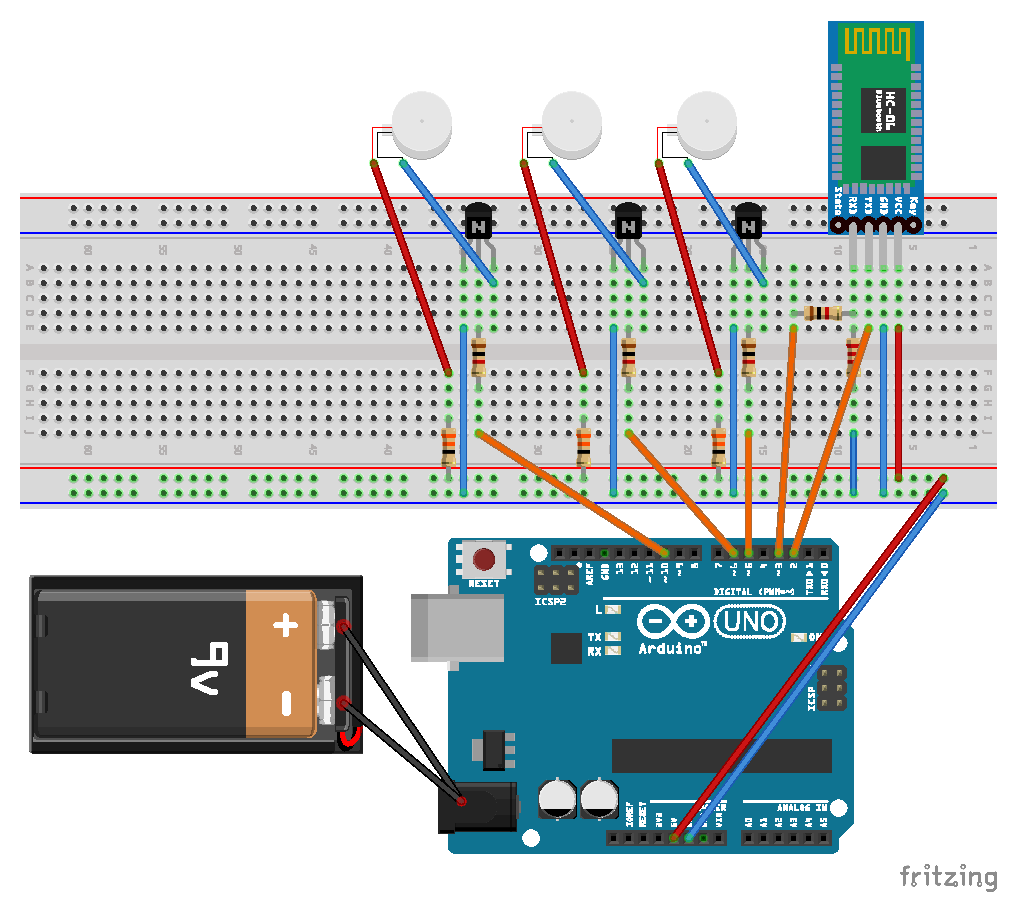
\includegraphics[width=0.75\textwidth]{images/circuit-design_bb.pdf}
    \caption{Figure shows the outlined work plan, visualised as a Gantt chart. Large tasks are divided into smaller deliverables. Time is split into weekly intervals.}
    \label{fig:work-plan}
\end{figure}


\subsubsection{Bike Radar Design}
On the other side of the TactiHelm system is the Garmin Varia RTL515 bike radar \cite{garminradar}. Designed to attach to the back of a bicycle, the radar can detect vehicles up to a range of 140 metres, with a viewing angle of 220\degree{}. The radar allows for two communication methods: Bluetooth Low Energy (BLE) and ANT+. Communicating using BLE provides us with access to the distance and speed of each detected vehicle. Notably, BLE does have limitations such as a smaller bandwidth compared to ANT+ \cite{bluetoothlimitations}. However, this is not a concern since only a relatively small amount of data is being transferred. From this, the following questions remain:
\begin{itemize}
    \item Which metric (or metrics), from distance, speed, or some arbitrary combination of the two, is most suitable for signifying an approaching vehicle to a user?
    \item How can this metric be conveyed to a user? Should continuous values be encoded, or should the metric be defined into categories? What do these arbitrary categories mean to users? 
    \item How can this information be encoded using vibro-tactile cues?
\end{itemize}
Answers to such questions are explored with a lab-study investigating different cues and encodings, described in Section \ref{sec:lab-study}.


\subsubsection{App Design}
To allow communication between the bike radar, and Arduino, a custom-built React Native application was developed, to act as a mediary between the two devices, as seen in Figure 2. The current state of the application can run on an Android mobile phone; however, future versions of the app would ideally also run on an iOS device. Currently, the following functionality is possible with the application:
\begin{itemize}
    \item Connect to the HC-06 Bluetooth module using Bluetooth Classic
    \item Connect to the Garmin Varia using Bluetooth Low Energy
    \item Receive the distance and speed information of each detected vehicle from the bike radar.
    \item Manually turn on/off and control the vibration intensity of each connected actuator.
\end{itemize}

What remains to be implemented is a pipeline between the bike radar and Arduino. More specifically, the information received via BLE from the bike radar should be parsed and encoded into the relevant vibro-tactile cues. However, this is not possible, until such encodings to cues are defined, as discussed further.


\subsection{Exploratory Survey}\label{sec:survey}
To identify the requirements of a hazard notification system such as TactiHelm, an online survey was conducted to understand cyclists' attitudes and behaviours towards safety while cycling. The survey used a mixture of open response, Likert scale, and multiple choice questions to explore topics such as use of safety equipment and techniques and causes of injuries. It was distributed to various cycling groups around Glasgow, and respondents were urged to answer as truthly and honestly as possible. We emphasised that we did not intend to judge any participants' answers on their safety, legality, or 'sensibility' - instead we only wish to gather insights for use for the project.

The survey was answered by 110 respondents, aged from 16-24 (14.55\%), 25-34 (10.91\%), 35-44 (11.82\%), 45-54 (31.82\%), 55-64 (24.55\%) and 65+ (5.45\%) years old. Participants identified as 61.82\% male, 37.27\% female, and 0.91\% non-binary. Finally, roughly 90\% of respondents were from Scotland, with the majority from Glasgow. This demographic data was collected as studies has shown that the risk and severity of cyclist injury vary depending on factors such as roadway characteristics and demographic group \cite{BEHNOOD201735}.

90\% of respondents answered saying they cycle more than one hour a week, with 42.73\% of respondents cycling 7+ hours a week. Respondents equally cycled on city roads (30.37\%), cycle paths (29.63\%), and country roads (28.15\%), with the remaining 11.85\% cycling in other environments. Notably, 72.73\% of respondents answered that they had suffered some kind of injury while cycling - 60\% a minor injury and 12.73\% a major injury. Reasons for injury varied, from slipping on wet and uneven roads, to colliding with another road vehicle.

When asked about their usage of a helmet, over 80\% of participants stated that they regularly wear one. When asked for reasons for not wearing a helmet, a variety of responses were given, with the most common being that they are not available when hiring a bike. Interestingly, some respondents answered that they did not believe helmets to be useful in certain scenarios, \textit{“Helmets are designed to prevent injury at relatively low speeds, speeds which are comfortably exceeded by adult cyclists of even moderate fitness. I believe the effectiveness of helmets to prevent injury is grossly overstated”} [P13]. However, multiple studies conducted on the effectiveness of bicycle helmets \cite{10.1093/ije/dyw153, HOYE201885, HOYE2018239, buth2023effectiveness} have found that regardless of the crash severity, helmets can help reduce the severity of head injuries by 48\% \cite{HOYE201885}.

When asked about safety technology, the most common equipment following from a helmet were cycle lights (87.27\%), reflective gear (64.54\%), and bike computer or mounted smartphone (60.90\%). Of nine respondents who stated they had a bike radar, all of them said they had a Garmin radar. When asked to comment on its usefulness they all expressed that they benefit from being more aware of vehicles behind them; however, a common disadvantage is its high cost.

Participants were asked to freely respond with the challenges they face which makes cycling feel unsafe. Categorising the responses, the most common ones were \textit{“close passes from cars”} (38.18\%), followed shortly by \textit{"poor cycling infrastructure”} (34.54\%).

Finally, participants were provided with a brief description of TactiHelm and were invited to comment on its usefulness for cycling. Respondents thought the concept could be useful, but were worried that it may be distracting - expressing concern that it may remain vibrating at all times while a vehicle is detected. These comments are useful in understanding users pre-conceived notions and worries as to how such as system may operate, and help shed light on specific problems which should be addressed in TactiHelm.


\subsection{Lab Study - Investigating Vibro-tactile Distance Encodings}\label{sec:lab-study}
A key idea which remains to be investigated is how a given metric can be encoded using vibro-tactile cues to effectively warn a cyclist of an approaching vehicle. The following section details a future lab-study to be conducted, to explore how distance can be effectively encoded for our system. Distance is chosen as it is assumed to be the most appropriate metric for the described system.

\subsubsection{Chosen Parameters}
As previously mentioned in Section \ref{sec:coding-distance}, a vibro-tactile display affords four parameters which can be adjusted: the location, timing, frequency, and amplitude of a vibration \cite{guidelines}. In our described system, the \textit{'intensity'} of a vibration is controlled by varying the voltage to the motor using pulse-width-modulation (as described in Section \ref{sec:helmet-design}). These changes in voltage results in simultaneous changes in frequency and amplitude, meaning the parameter \textit{'intensity'} is treated as a combination of these two parameters. However, whether these are suitable parameters for our system depends on how many intervals we wish to categorise distance, as frequency and amplitude only have 5-7 perceptually distinguishable levels \cite{guidelines}. From this, and additionally for the sake of simplicity, we choose not to study how the intensity can be varied. 

This leaves the parameters of location and timing to be used to encode distance. Many studies have investigated how timing (or more specifically, rhythm) can be used to represent different distances \cite{10.1145/1060581.1060585, 5326374, 10.1145/1520340.1520718, 10.1145/1753326.1753581, 10.1145/1868914.1868923}. In these studies, the distance is typically measured from a moving wearer, to a stationary point of interest (POI), where the wearer is moving towards the POI. However, in the context of our described system, the POI (the approaching vehicle) is moving towards the wearer, who is also travelling in the same direction. This motivates the need to study whether typical rhythm coding schemes for distance are still appropriate for use in our described context.

Furthermore, no studies to the best of our knowledge have investigated how the location of a vibration can convey distance. This is likely because the location parameter is typically used to convey direction. However, a unique feature the use of a helmet affords is the ability to use locations across various anatomical planes. That is, the sagittal, coronal, and axial planes \cite{anatomical}. In the context of vibro-tactile systems, motors on a belt-based display [cite all belt displays] would be considered to be along the axial plane, whereas motors on a vest display [cite all vests] or split along both wrists [cite], would be considered to be along the coronal plane. However, no studies to the best of our knowledge have investigated how vibro-tactile motors can be used to convey information across the sagittal plane.

From this, our lab-study presents the opportunity to provide three novel contributions regarding distance encoding schemes.
\begin{enumerate}
    \item Is the typical use of rhythm to encode distance, a suitable parameter in the context of a hazard awareness system for approaching vehicles from behind?
    \item How can the sagittal plane be utilised for vibro-tactile displays?
    \item Is location of a vibration a suitable parameter to encode distance?
\end{enumerate}


\subsubsection{Procedure}\label{sec:lab-procedure}
The first phase of the study is to investigate different location coding schemes for distance. Three schemes have been defined for study. Notably, for each scheme, the intensity and rhythm is kept constant:
\begin{enumerate}
    \item Singular Vibration - only the tactor at the location relative to the specified distance is activated.
    \item Sequential Synchronous Vibration - all tactors up to the tactor at the location relative to the specified distance are activated at the same time.
    \item Sequential Asynchronous Vibration - all tactors up to the tactor at the location relative to the specified distance are activated one at a time in sequential order.
\end{enumerate}
These schemes will be tested on recruited participants to investigate which scheme participants find best at conveying distance. We hypothesise that participants will prefer the asynchronous vibration scheme, as this utilises the vibro-tactile illusion of sensory saltation \cite{5710913}. Additionally, we predict that participants may experience the illusion of funneling when using the synchronous scheme, due to the simultaneous activation of tactors. NUMBER AND SPACING OF TACTORS for the reason of funneling.

The second phase of the study is to investigate different rhythm coding schemes for distance. Three schemes have been defined for study. Notably, for each scheme, the intensity and location is kept constant. Specifically, the location is the singular tactor in the occipital region, as this points in the direction of the approaching vehicle.
\begin{enumerate}
    \item Monotonic (delay-based) - the activation delay continuously decreases as distance decreases.
    \item Categorical (duration-based) - the duration of the rhythm (the number of pulses) decreases as the distance decreases.
    \item Hybrid - a multi-phase model, which is categorical while the distance is far, but once a vehicle is imminent, it switches to a monotonic scheme.
\end{enumerate}
These schemes will be tested similarly to how the location schemes are. The monotonic encoding is inspired from van Erp et al. \cite{10.1145/1060581.1060585}, who compared different rhythm coding schemes for waypoint navigation. Specifically, an absolute encoding is used, where the delay decreases by a specific amount every $x$ amount of meters (compared to a relative encoding which decreases the delay be a percentage of the distance left). The categorical encoding is inspired from Asif et al. \cite{10.1145/1868914.1868923}, who compared different rhythm encodings, finding that participants found the combination of rhythm and duration the best at conveying distance. The hybrid encoding is inspired by Steltenpohl and Bouwer \cite{10.1145/2449396.2449450}, who combined two schemes similar to the described monotonic and categorical ones, to create a two-phase rhythm and duration distance encoding.

Although arguably, these rhythm encodings could be further refined into more schemes; for instance, another definition of a hybrid scheme may decrease the activation delay when the distance category changes, or the monotonic scheme could be divided into a relative and an absolute scheme. This is simply meant to serve as an initial study investigating how rhythm can be used to encode distance for a hazard awareness system. Future work would ideally investigate such further refined schemes.

The final phase of the study is to compare the location and rhythm schemes to conclude which one is best for our given system. We hypothesise that the combination of the best location and rhythm encoding, will produce the most ideal scheme.

\subsection{User Study - TactiHelm Evaluation}\label{sec:user-study}

%%%%%%%%%%%%%%%%%%%%%%%%%%%%%%%%%%%%%%%%%%%%%%%%%%%%%%%%%%%%%%%%%%%
\section{Work Plan}
As discussed in the previous section, at the current stage of the project, we have achieved the following:
\begin{itemize}
    \item Conducted a user survey to gather an initial understanding to cyclists' thoughts and beliefs regarding safety while cycling.
    \item Developed a mobile application which can connect to our bike radar and Arduino, and has remote control over each tactile actuator.
    \item Thoroughly planned two studies to investigate distance coding schemes and then evaluate our finished TactiHelm product.
\end{itemize}
What remains to be done is to, prepare for, conduct, and then analyse the results of each study. Finally, we then must write our final article. This chapter outlines the intermediate deliverables and dates needed to complete the project. For simplicity, the plan is divided into weekly intervals, between the 8\ts{th} January and the deadline of April 12\ts{th}. The whole plan is detailed in a Gantt chart as shown in Figure x.

The first large stage of work to be completed is the lab study as detailed in Section \ref{sec:lab-study}. This stage is expected to last from 08/01/24 to 05/02/24. Described below are the intermediate deliverables needed to complete this stage, and their expected dates: 
\begin{enumerate}[label=1.\arabic*]
    \item Prepare materials for study (08/01 - 15/01): before the study can be conducted, we first need to recruit participants, create briefs and debriefs, and plan a space to perform the study, among other preparations.\label{task:lab-prep}
    \item Design cues (08/01 - 22/01): the relevant vibro-tactile cues to be evaluated in the study need to be designed (as discussed in Section \ref{sec:lab-procedure}). These should be able to be activated from the mobile app on command. \label{task:lab-cues}
    \item Conduct study (22/01 - 29/01): the study can be performed with participants over the course of a week. This task is dependent upon tasks \ref{task:lab-prep} and \ref{task:lab-cues}. \label{task:lab-conduct}
    \item Analyse results (29/01 - 05/02): the results from the study need to be analysed, in-order to understand which encoding scheme for distance is most suitable. This task is dependent upon task \ref{task:lab-conduct}.
\end{enumerate}

The next large stage is to use the results gathered from the labs study, to design a real-world user study to evaluate our final TactiHelm product. This stage is expected to last from 05/02/24 to 11/03/24. Described below are the intermediate deliverables needed to complete this stage, and their expected dates: 
\begin{enumerate}[label=2.\arabic*]
    \item Prepare materials for study (05/02 - 12/02): before the study can be conducted, we first need to recruit participants, create briefs and debriefs, and plan a space to perform the study, among other preparations.
    \item Create pipeline from radar to cues (05/02 - 19/02):
    \item Additional bug fixing (19/02 - 26/02):
    \item Conduct study (26/02 - 04/03):
    \item Analyse results (04/03 - 11/03)
\end{enumerate}

The final large stage of work to be conducted is to write our final article piece. This stage can run concurrently alongside the other stages, and is expected to last from 12/02/24 to 01/04/24. This provides a buffer period of 11 days for potential changes and problems.

\begin{figure}[!ht]
    \centering
    \includegraphics[width=1\textwidth]{images/work-plan.pdf}
    \caption{Figure shows the outlined work plan, visualised as a Gantt chart. Large tasks are divided into smaller deliverables. Time is split into weekly intervals.}
    \label{fig:work-plan}
\end{figure}


%%%%%%%%%%%%%%%%%%%%%%%%%%%%%%%%%%%%%%%%%%%%%%%%%%%%%%%%%%%%%%%%%%%
% it is fine to change the bibliography style if you want
\bibliographystyle{plain}
\bibliography{interim}
\end{document}
